\subsection{TAOCP 7.1.1 exercises 4 and 5}

Found this exercise in \href{http://www.cs.utsa.edu/~wagner/knuth/fasc0b.pdf}{TAOCP section 7.1.1 (Boolean basics)}:

\begin{figure}[H]
\centering
\frame{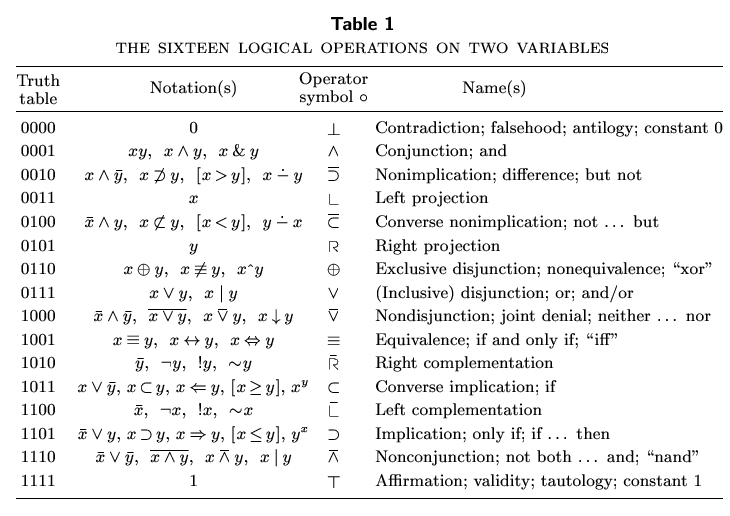
\includegraphics[scale=0.7]{logic_synth/TAOCP_711_4_and_5/page3.png}}
\caption{Page 3}
\end{figure}

\begin{figure}[H]
\centering
\frame{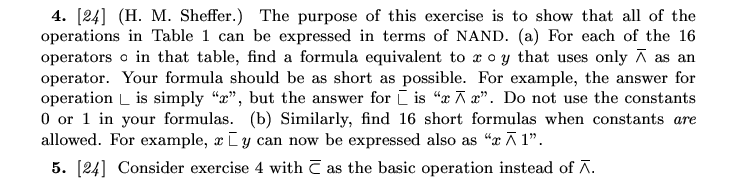
\includegraphics[scale=0.7]{logic_synth/TAOCP_711_4_and_5/page34.png}}
\caption{Page 34}
\end{figure}

I'm, not clever enough to solve this manually, but I could try using logic synthesis, as I did before.
As they say, "machines should work; people should think".

The modified Z3Py script:

\lstinputlisting[style=custompy]{logic_synth/TAOCP_711_4_and_5/logic_for_TAOCP.py}

My solution for NAND:

\lstinputlisting{logic_synth/TAOCP_711_4_and_5/nand.txt}

My solution for NAND with 0/1 constants:

\lstinputlisting{logic_synth/TAOCP_711_4_and_5/nand_constants.txt}

My solution for ANDN:

\lstinputlisting{logic_synth/TAOCP_711_4_and_5/andn.txt}

My solution for ANDN with 0/1 constants:

\lstinputlisting{logic_synth/TAOCP_711_4_and_5/andn_constants.txt}

Correct answers from TAOCP:

\begin{figure}[H]
\centering
\frame{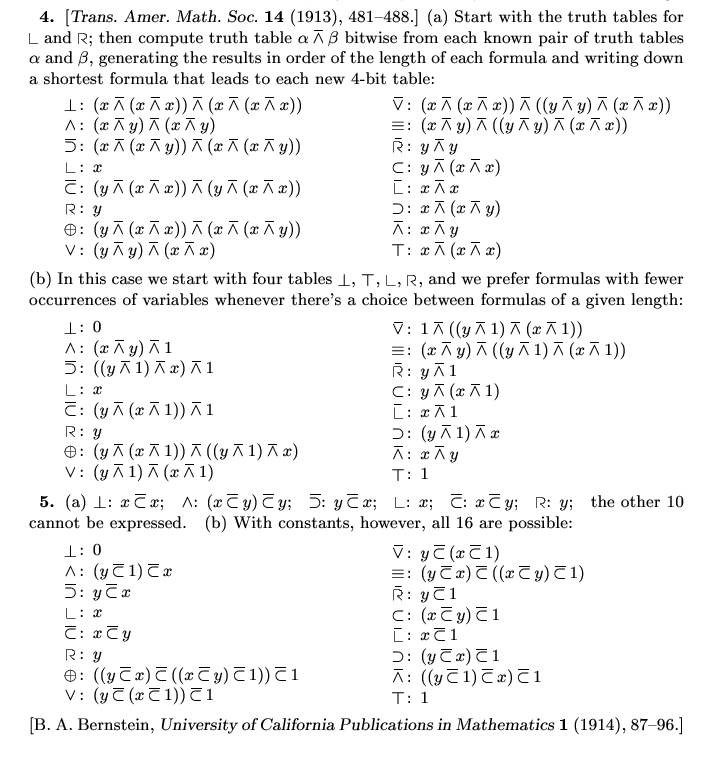
\includegraphics[scale=0.7]{logic_synth/TAOCP_711_4_and_5/page51.png}}
\caption{Page 51}
\end{figure}

My solutions are slightly different: I haven't "pass through" instruction, so sometimes a value is copied from the input to the output using NAND/ANDN.
Also, my versions are sometimes different, but correct and has the same length.

